\subsection{Серверное ПО и лицензирование}

Для работы программных пакетов, представленных в задании на разработку, необходима ОС
семейства Windows. Также, необходима ОС, позволяющая многопользовательскую работу, то
есть Windows Server. Актуальная на момент разработки версия — Windows Server 2019. У
данной версии есть три варианта: Essentials, Standart и Datacenter.
\cite{ref:win_srv_comp}\cite{ref:win_srv_overview}.

\begin{enumerate}
    \item Datacenter ‒ предназначен для развёртывания в облачных средах и в центрах по
        обработке данных при высоком уровне виртуализации. Лицензия приобретается по
        принципу: одна лицензия \say{на ядро} (core-based);
    \item Standard ‒ ориентирована для использования в среде с минимальными уровнями
        виртуализации, а также в физической среде. Лицензирование производится так же,
        как и в случае с \say{Datacenter};
    \item Essentials ‒ редакция, ориентированная на малый бизнес, с ограничением на
        количество клиентов — допускается не более 50 устройств и максимум 25
        пользователей. Данная редакция получает лицензию по методу server-based:
        один физический сервер – одна лицензия (на каждый дополнительный сервер
        необходимо приобретать новую лицензию).
\end{enumerate}

Подробное сравнение этих вариантов приводится в таблице~\ref{tab:win_srv_comp}.
Также стоит отметить, что для многопользовательской работы в редакциях Standart и
Datacenter необходимо покупать дополнительные лицензии для каждого клиента. Такие
лицензии называются Client Activation License (CAL).

\begin{table}[h]
    \centering
    \caption{Сравнение редакций Windows Server 2019}
    \label{tab:win_srv_comp}
    \begin{tabularx}{\linewidth}{XXXX}
        \toprule
        Редакция & Essentials & Standart & Datacenter \\
        Лицензирование & На сервер & На ядро + CAL & На ядро + CAL \\
        Виртуализация & Да & Да; 2 виртуальные
        машины и один узел Hyper-V на лицензию & Да; неограниченное количество
        виртуальных машин и один узел Hyper-V на лицензию. \\
        Защищенные виртуальные машины & Нет & Нет & Да \\
        Программные сетевые интерфейсы & Нет & Нет & Да \\
        Программное хранилище данных & Нет & Нет & Да \\
        \bottomrule
    \end{tabularx}
\end{table}

Исходя из этих ограничений, можно выбрать редакцию Essentials для разрабатываемого
проекта. Ограничения касаются в основном функций виртуализации, которые в данном проекте
не используются.

\subsection{Выбор используемого протокола}

Для разработки необходимо выбрать способ удаленного доступа, который будет
использоваться в системе. Так как выбор зависит от серверной ОС, выбор оптимального
варианта связан с доступными на Windows протоколами.

Основной протокол, используемый в Windows — RDP (Remote Desktop Protocol). Клиент RDP
доступен во всех редакциях Windows, начиная с Windows XP, что позволяет использовать
любой компьютер кафедры в качестве тонкого клиента (см. рисунок \ref{pic:mstsc_xp}).
Однако, RDP-клиенты существуют для многих платформ, в том числе для Linux.

\begin{figure}[h]
    \center
    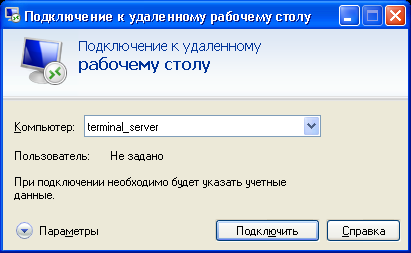
\includegraphics[height=8cm]{mstsc_xp}
    \caption{Окно RDP-клиента, встроенного в Windows XP}
    \label{pic:mstsc_xp}
\end{figure}

\subsection{Клиентское ПО}

В качестве клиентской ОС выбран стандартный для Raspberry Pi дистрибутив Linux Raspbian,
основанный на Debian \cite{ref:raspbian}.
Дистрибутив поддерживается Raspberry Pi Foundation и рекомендован к установке.
К его преимуществам можно отнести открытый исходный код, простоту установки и удобство 
настройки. 
Актуальной на момент разработки была версия Buster, вышедшая в феврале 2020 года.

Для RDP-клиента использовано ПО \textit{FreeRDP}, актуальной на момент разработки версии
2.0.0 \cite{ref:freerdp}. Данный программный продукт позволяет осуществлять подключение
к RDP-серверам любой версии, просто и гибко настраивается для получения оптимальной
производительности.  Так как исходный код открыт, есть возможность скомпилировать
бинарный файл для нужной архитектуры (в рассматриваемом проекте используется архитектура
ARM).

